\section{Data Needed}
In order to create a suitable database schema for the database that want to create, we first need to figure out what will be in the database. This analysis will focus on the structure of the institutions involved in the GIRAF project. \autoref{fig:data_overview} illustrates the relationship between the various departments and people involved in the institutions.

First of all there can be several departments of an institution. Each department has an administrator and each department can have some subdepartments. Each department has a number of employees, which will be referred to as guardians, assigned to it as well as some children that attend the department. Each guardian is responsible for a few specific children, but is of course not limited to only taking care of to ones he is responsible for. 

\begin{figure}
	\begin{center}
	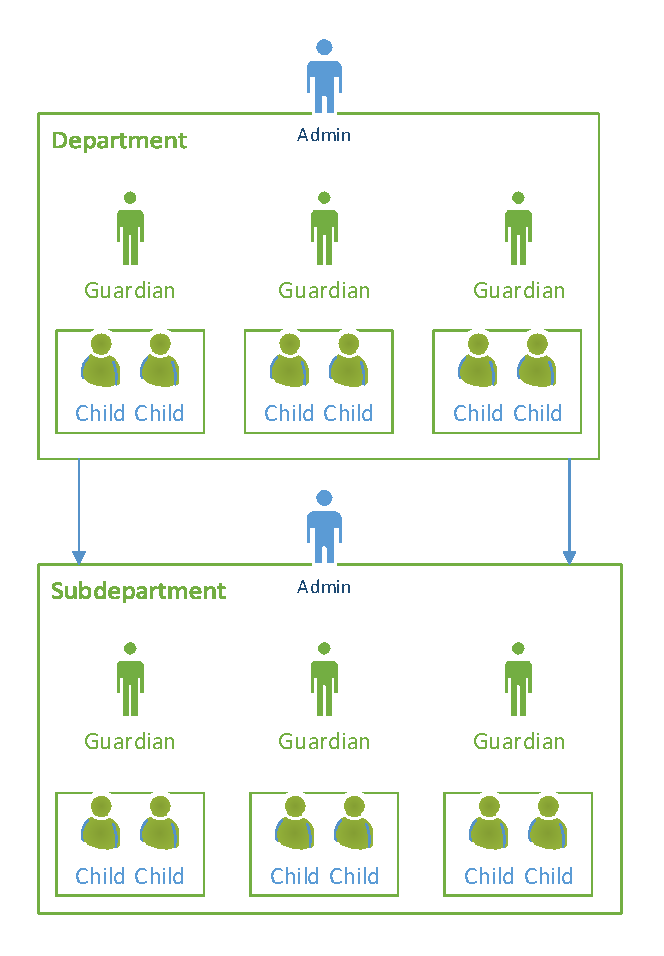
\includegraphics[width=0.5\textwidth]{img/data_overview.pdf}
	\end{center}
	\label{fig:data_overview}
	\caption{Overview of the people involved and department structure}
\end{figure} 

The children have some needs and demands that can vary greatly from one child to another. But common for all of the children is that they each have their own set of pictograms. The children generally have a resistance to change e.g. the taxi that drives them to the institution and picks them up again has to have a specific color. This tendency can also occur with regard to preferences as some children insist on their pictograms being black on white with stick figure and other might prefer colored images. 

If we try to apply these things to what could be used in the database schema, we need to be able to represent \emph{department} with optional \emph{subdepartments} we also need an \emph{administrator} that can be assigned to the departments. There needs to be able to representation of \emph{guardians} and \emph{children}. The \emph{pictograms} might also need to be included and it might be a good idea to be able to categorize the pictograms e.g. cereal and milk under breakfast items.

\begin{figure}
	\begin{center}
	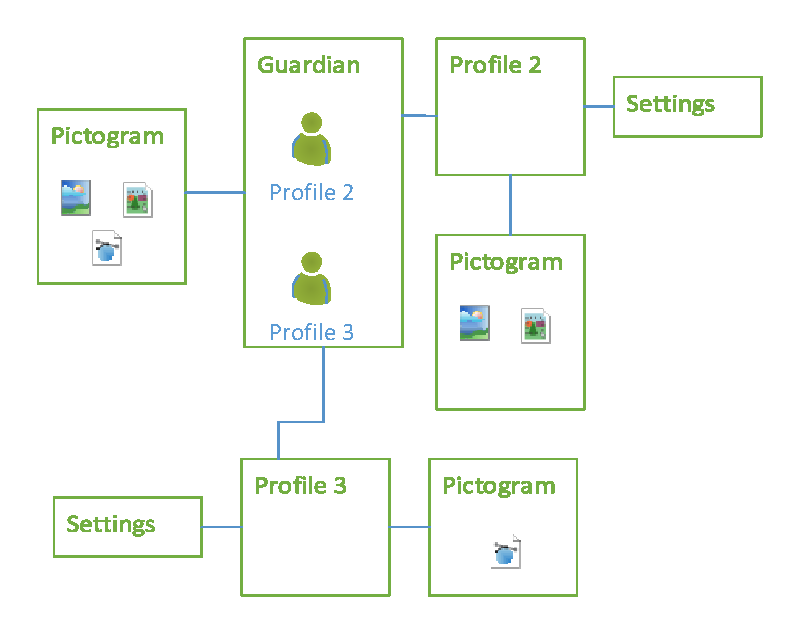
\includegraphics[width=0.5\textwidth]{img/child_guardian.pdf}
	\end{center}
	\label{fig:child_guardian}
	\caption{Illustration of the relationship between guardian and children}
\end{figure} 

It might be a good idea to start with a profile entity that can cover over both children and guardians. A specific profile could then be guardian of a number of other profiles. If a profile is not guardian of other profiles then it is a child profile. The profile can have his own preferences in games and have a custom set of pictograms. And will of course be assigned to a department. \autoref{fig:child_guardian} illustrates this relationship where profile 1 is the guardian of profiles 2 and 3. All of the profiles have their own set of pictograms assigned to them and profile 1 as guardian has the authority to edit in it's children's pictograms.


